\section{Introduction}
\label{sec:maggie_introduction}

\newcommand\rvir{r_{\rm vir}}
\newcommand\vvir{v_{\rm vir}}

We show in the last chapter that the most used galaxy group algorithm that is
the FoF should be optimized against its linking lengths, and that it depends on
the scientific goal of the group catalog obtained. With these limitations, it
is clear why Bayesian methods appeared. Indeed, with our knowledge of the
galaxy formation and evolution processes, it is possible to constrain better
the galaxy grouping. With the FoF algorithm, galaxies are selected in a pure
geometrical way, and their formation history doesn't matter in this selection,
since only the over-density is relevant. With Bayesian algorithms, it is
possible to combine geometrical and physical approaches. The history of
galaxies is available by their observable properties such as luminosity,
stellar mass, morphology and is used to assign galaxies to a group, in
complement of the geometrical information from the density. In particular, a
galaxy can be rejected of a group selected by density criterion if its
properties don't reflect the history it would have inside this group.

We already described Bayesian algorithms in
\bartrefchapter{galaxy_group_algorithms}, for example \citet{Yang+07} or
\citet{MunozCuartas+12}, where similar spatial methods to the FoF are adopted,
with priors as the density profile of galaxies inside halos to constrain the
assignation. But because of observational uncertainties, model divergences,
various incompletenesses\ldots, the extraction of groups from observational
data will always be affected by these problems, and the galaxy environment
polluted by interlopers, creating biases in group characteristics. This leads
to bad modulation of galaxy properties with their environment and a
falsification of our understanding of intra-groups physical processes.

Recently, with the improvement of computer capacities in terms of memory and
power, it becomes possible to include many priors in the computation, and to
use the most computation intensive applications of statistics. Since
interlopers will still be problematic, the new powerful computer era allowed
probabilities to describe the membership of galaxies in groups. Systematic
errors in galaxy surveys can be reduced or integrated in the grouping by
probabilities. For example, \citet{Liu+08} used a probabilistic FoF in galaxy
survey with photometric redshifts to avoid the uncertainties inherent to this
method. \citet{DominguezRomero+12} also used responsibilities to improve the
assignation of galaxies to groups and reduce interlopers effect on their
observable properties. In \citet{Rykoff+14}, galaxies have their probabilities
based on the group richness estimations.

It seems that using probabilities to describe the membership inside galaxy
groups will be inevitable, because of the systematic errors and biases presents
in the actual and future galaxy surveys. In particular, the modulation of the
galaxy properties with their environment that we want to extract from galaxy
group catalogues should be less biased by interlopers if we use probabilities
as a weight. Indeed, interlopers, even if they are still present in the group
membership, will have a low probability to pertain to the group, and their
contribution to galaxy group properties reduced.

Here is the starting point of our galaxy group algorithm called MAGGIE\@:
Models and Algorithm for Galaxy Group, Interloper and Environment. We combine
our understanding from the galaxy formation, using various models, to compute a
probability for galaxies to belong to a peculiar group, and use it in the
algorithm for the group extraction. Then interloper effects should be reduced
in the characterization of the environment.

In the following sections, we will describe the algorithm and its
implementation, the application to the SDSS and show its limitations.

\section{Algorithm}
\label{sec:algorithm}

\subsection{Description}
\label{sub:maggie_description}

MAGGIE doesn't affect a galaxy to an unique group, but it affects a probability
for this galaxy to be in a group. With this principle, a galaxy is possibly
assigned to more than one group. It's the goal of MAGGIE\@: to obtain the
properties of galaxy groups in statistical and probabilistic senses. This
allows users of catalogues generated by MAGGIE to compute some properties of
groups taking into account the fact that a galaxy could not be assigned
arbitrarily to one group with some criteria of affectation. But the most
important, it's that this probability contains the information of being an
interloper or not.

MAGGIE is organized in an iterative way in order to be self-consistent with
the data being analysed, as for learning algorithms. For this reason, we
will describe the implementation of the algorithm in different steps. In
what follows, we assume that we have a galaxy sample with
positions (right ascension RA, declination DEC), redshifts, stellar masses,
apparent magnitudes in a given band and absolute magnitudes. It's the
minimum set of data necessary.
%
\begin{enumerate}
    \item We first get some potentials groups in order to have a \emph{seed} in
        the iterative process. For this, we make an assumption: the most
        massive galaxies (in stellar mass) are potential group centers. In an
        other implementation, we use the luminosity of the central (the reason
        is explained in \bartrefsubsection{observational_errors}). But, some
        intra-group physical process can lead to a false detection of the
        brightest galaxy as the central one \citep{Ebeling+13}. From the galaxy
        sample, we sort by decreasing stellar mass (or luminosity) all galaxies
        and we start with the most massive (most luminous) as centre of a
        potential group.

    \item\label{step:2} For all our potential groups, we need to get our
        potential members. We are just interested in the virial sphere of
        groups. Since the unique information on groups at this step is the
        central galaxy, we use its stellar mass (or luminosity). At first
        iteration, we use the relation between halo mass and central stellar
        mass from \citet{BCW+10} (and a simple ratio relation for luminosity).
        We used other models later to see the influence of this choice (see
        \bartrefsubsection{prior_relation}). For next iterations, we use the
        same relation, but learned from our previous iterations. We can
        estimate the virial radius of the group assuming that the halo mass
        corresponds to the virial mass. Then, we select all galaxies in a cone
        generated by an angular separation corresponding to the virial radius
        physical size at the group's redshift (the redshift of the central
        galaxy).

    \item With group membership, we compute galaxy probabilities to belong
        to it. The probability is computed assuming a density profile of
        galaxies in groups, and a velocity distribution. Considering that
        galaxies form in dark matter halos, the density profile of
        galaxies in groups must follow a NFW distribution \citep{NFW+97}
        which fit remarkably well the dark matter particles distribution in
        $\rm \Lambda$CDM simulations. The detailed computation of the
        probability is provided in \bartrefsection{probability}.

    \item We compute the weighted (by probability) stellar mass and luminosity
        of groups. For this we use a probability threshold $p_{\min}$ to decide
        if a galaxy is associated to a group, i.e.\ if we take the galaxy for
        the estimation of the group stellar mass and luminosity. This parameter
        will be optimized by tests. The way of computing this properties for a
        group is the following: we sum, using the probability weights,
        luminosities and stellar masses of galaxies that have an absolute
        magnitude less than the limit magnitude defined by the sample, in order
        to be complete.

    \item Using the stellar mass of the central galaxy, we can estimate the
        halo mass of the group. We use the abundance matching technique which
        assumes that there is a one-to-one relation between the central stellar
        mass of the group and its halo mass. It allows to compare the
        cumulative distribution function (CDF) of the two quantities. Indeed,
        with this assumption, the number of groups above a given central
        stellar mass (or luminosity) is the same than the number of groups
        above the corresponding halo mass. If we consider a certain halo mass
        function, we can predict the halo mass of a group with a given central
        stellar mass (or luminosity) by comparing the CDF of the data with that
        predicted by the halo mass function.

    \item With the halo mass found for group by this abundance matching, we
        go back to step~\ref{step:2} and recompute groups with the halo
        mass-central stellar mass relation previously obtained. This process
        goes until there is a convergence in the number of groups.
\end{enumerate}

If we follow this schema, there will be as many groups as galaxies. To avoid
the inherent fragmentation introduced by this method, we used an other
threshold probability to reduce the number of groups. We allow a galaxy to be a
central galaxy only if its probability to belong to an other group (already
determined in the loop for potential galaxy groups) is smaller than the
threshold $p_{\max}$. For this comparison, we consider the probability that is
maximal in all groups the galaxy is in. In this way, we exclude while iterating
over potential groups a large number of central galaxies, and avoid the
fragmentation.

\section{Probability}
\label{sec:probability}

The probability is one of the most important aspect of MAGGIE\@. Since the
observer study galaxy groups only in the projected phase space (hereafter
\emph{pps}), for defining the probability, we consider the location in
the \emph{pps} of the group with its projected radius $R$ and the
line-of-sight velocity $v_z$. The probability to be member of the halo or
not at a given location, is the number of cases where we are inside the halo
relatively to the total number of cases. The \emph{pps} density $g$ is this
definition of ``number of cases''. We can write our probability $p$ to be in
the halo as:
%
\begin{equation}
    \label{eq:probability}
    p \left(R, v_z\right)= \cfrac{g_h \left(R, v_z\right)}
    {g_h \left(R, v_z\right) + g_i \left(R, v_z\right)}
\end{equation}
%
where $g_h$ is the projected density inside the group and $g_i$ is the
background density, i.e.\ the interloper density.

In \bartrefsubsection{general_case}, we describe how to compute the
probability with a general density profile and then in
\bartrefsubsection{analytical_forms} some analytical forms
available with some models.

\subsection{General case}
\label{sub:general_case}

To compute the projected density of galaxies in the halo we have to assume some
models for their phase space distribution. So we use the distribution function
$f$ of the system:
%
\begin{equation}
    f\left(\textbf{r},\textbf{v}\right)\dd\textbf{r}\dd\textbf{v}
    =\rho\left(r\right)\dd{x}\dd{y}\dd{z}
    h\left(\textbf{v}\right)
    \dd v_r\dd v_\theta\dd v_\phi=
    \dd^6 N
\end{equation}
%
where $h\left(\textbf{v}\right)$ is the velocity distribution of galaxies in
the halo.

If we consider the line of sight as the axe of cylindrical coordinates, we
can write:
%
\begin{equation}
    f\left(\textbf{r},\textbf{v}\right)\dd\textbf{r}\dd\textbf{v}=
    \rho\left(r\right)R\dd{R}\dd\phi\dd{z}h\left(\textbf{v}\right)
    \dd{v_r}\dd{v_\theta}\dd{v_\phi}
\end{equation}

By definition, the projected phase space density is just the number $N$ of
galaxies with their \emph{pps} coordinates in the ring defined by the range
$R+\dd R$ and $v_z+\dd v_z$.
%
\begin{equation}
    g_h \left(R, v_z\right)2\pi R \dd R \dd v_z = \dd^2 N
\end{equation}

We can see that $r^2=z^2+R^2$, so $\dd{z}=r/\sqrt{r^2-R^2}\dd{r}$.
Now, to have the projected density on the sphere, we just need to integrate
over the line of sight and angles:
%
\begin{equation}
    \label{eq:intfunc}
    \int_0^{2\pi}\int_{z=-z_{\max\left(r\right)}}^{z_{\max\left(r\right)}}
    f\left(\textbf{r},\textbf{v}\right)\dd\textbf{r}
    \dd{\textbf{v}}=2\int_{r=R}^{r_{\mathrm{vir}}}2\pi
    \frac{r\rho\left({r}\right)}{\sqrt{r^2-R^2}}{R}\dd{R}\dd{r}
    {h\left({\textbf{v}}\right)}\dd{v_r}\dd{v_\theta}\dd{v_\phi}
\end{equation}

We need to integrate on the velocities too in order to get the line-of-sight
component, and retrieve the pps. For velocities, we make a transformation of
coordinates: we pass to spherical coordinates to the coordinates defined in
XX\@. The rotation matrix between both coordinates system is:
\begin{equation}
    \begin{pmatrix}
        v_r \\
        v_\theta \\
        v_\phi \\
    \end{pmatrix}
    =
    \begin{pmatrix}
        \cos\theta & \sin\theta & 0 \\
        \sin\theta & \cos\theta & 0 \\
        0 & 0 & 1 \\
    \end{pmatrix}
    \begin{pmatrix}
        v_z \\
        v_1 \\
        v_\phi \\
    \end{pmatrix}
\end{equation}
%
so the Jacobian of the transformation is unity:
%
\begin{equation}
    \label{eq:intintfunc}
    \int_0^{2\pi}\int_{z=-z_{\max\left(r\right)}}^{z_{\max\left(r\right)}}
    \int_{-\infty}^\infty\int_{-\infty}^\infty
    f\left(\textbf{r},\textbf{v}\right)\dd\textbf{r}\dd\textbf{v}=
    2\int_{r=R}^{r_{\mathrm{vir}}}2\pi
    \frac{r\rho\left(r\right)}{\sqrt{r^2-R^2}}R\dd{R}\dd{r}
    \tilde{h}\left(v_z\right)\dd{v_z}
\end{equation}
%
where $\tilde{h} \left(v_z\right) = \int_{-\infty}^\infty\int_{-\infty}^\infty
h \left(\textbf{v}\right)\dd v_1 \dd v_\Phi$

For simplifying the equations later, we use a normalization as in:
%
\begin{eqnarray}
    M(r)= &\int_0^r 4\pi x^2\rho \left(x\right)\dd x
        &=M_v{\overline{M}{(r/\rvir)}}\nonumber\\
    N(r)= &\int_0^r 4\pi x^2\nu \left(x\right)\dd x
        &=N_v{\overline{N}{(r/\rvir)}}\nonumber\\
    \rho\left(r\right)= &\cfrac{\dd M}{4\pi r^2\dd r}&=\frac{M_v}{4\pi \rvir^3}
        \overline\rho(r/\rvir)\nonumber\\
    \nu\left(r\right)= &\cfrac{\dd N}{4\pi r^2\dd r}&=
        \frac{N_v}{4\pi \rvir^3}\overline\nu (r/\rvir)\nonumber\\
\end{eqnarray}
%
where $a$ is the radius of slope -2 for the density profile in logarithm
scales, in other words the radius where:
%
\begin{equation}
    {\left.\cfrac{\dd \log \rho \left(r\right)}{\dd \log r}\right|}_{r=a} = -2
\end{equation}

With this normalization, we can write:
%
\begin{equation}
    g_h \left(R, v_z\right) =\cfrac{M_v}{\rvir^2}
    \cfrac{1}{2\pi}
    \int_{R/\rvir}^1
    \cfrac{x\overline\rho \left(x\right)}{\sqrt{x^2 -
    {\left(R/a\right)}^2}}\dd x \widetilde{h} \left(v_z\right)
\end{equation}

The density of interlopers is extracted from \citet{MBM+10} where:
%
\begin{equation}
    g_i\left(R,v_z\right)=\undemi g_i\left(R,|v_z|\right)=
    \undemi\left(A
        \exp\left[-\undemi{\left(\frac{v_z}{\sigma_i}\right)}^2\right]
    +B\right)\frac{M_v}{\rvir^2 \vvir}=
    \widetilde g_i\left(R,v_z\right)\frac{M_v}{{r_{\rm{vir}}}^2 v_{\rm{vir}}}
\end{equation}

\subsection{Analytical forms}
\label{sub:analytical_forms}

In the following, we will refer to different equations of the
\bartrefappendix{profiles}.

If we assume that the halos are at the dynamical equilibrium, the velocity
distribution of galaxies should follow a Gaussian distribution. This
assumption can be discussed \citep{Beraldo+14}.

In this case, the velocity distribution can be written:
\begin{equation}
    h\left(\textbf{v}\right)=
    \frac{1}{{\left({2\pi}\right)}^{3/2}\sigma_{\theta}^2\sigma_r}
    \exp\left(-\undemi\left(\frac{v_r^2}{\sigma_r^2}+
    \frac{v_{\theta}^2+v_{\phi}^2}{\sigma_{\theta}^2}\right)\right)
\end{equation}
%
assuming that we split the three components of the velocity into three
independent velocity distributions. We can transform:
%
\begin{equation}
    \label{eq:poly}
    \left(\frac{v_r^2}{\sigma_r^2}+\frac{v_{\theta}^2+
    v_{\phi}^2}{\sigma_{\theta}^2}\right) =
    a v_z^2 + b v_1^2 + c v_\phi^2 + 2 v_z v_1 d
\end{equation}
%
for the coordinate system defined in\note{Add figure for the system}
with:
%
\begin{eqnarray}
    a&=&\left(\frac{\cos^2\theta}{\sigma_r^2}+
        \frac{\sin^2\theta}{\sigma_\theta^2}\right)\nonumber\\
    b&=&\left(\frac{\cos^2\theta}{\sigma_\theta^2}+
        \frac{\sin^2\theta}{\sigma_r^2}\right)\nonumber\\
    c&=&\frac{1}{\sigma_\theta^2}\nonumber\\
    d&=&\left(\frac{1}{\sigma_r^2}-\frac{1}{\sigma_\theta^2}\right)\nonumber\\
\end{eqnarray}
%
Putting \bartrefequation{poly} to a canonical form and integrating
\bartrefequation{intfunc} over $v_\phi$ and $v_1$ we get:
%
\begin{equation} \tilde{h}\left(v_z\right) = \frac{1}{\sqrt{2\pi}\sigma_z}
\exp\left(-\undemi{\left(\frac{v_z}{\sigma_z}\right)}^2\right) \end{equation}
%
since:
%
\begin{equation} \sigma_z^2 =
\sigma_r^2\left(1-\beta{\left(\frac{R}{r}\right)}^2\right) \end{equation}
%
and $\beta$ is the anisotropy profile $\beta=1-\sigma_\theta^2/\sigma_r^2$.

Finally, the projected density of galaxies in a halo is:
%
\begin{equation} g_h \left(R, v_z\right) =\cfrac{M_v}{\rvir^2}
    \cfrac{1}{2\pi}
    \int_{R/\rvir}^1
    \cfrac{x\overline\rho \left(x\right)}{\sqrt{x^2 -
    {\left(R/\rvir\right)}^2}}\frac{1}{\sqrt{2\pi}\sigma_z}
    \exp\left(-\undemi{\left(\frac{v_z}{\sigma_z}\right)}^2\right)\dd x
\end{equation}

If we work with velocities in units of the virial velocity $v_v$, i.e.\
$\hat{v_z}=v_z/v_v$, the ratio between the interloper and halo \emph{pps}
density is:
%
\begin{equation}
    \label{eq:gi_over_gh}
    \frac{g_i}{g_h}\left(R,v_z\right)=
    \frac{{\left(2\pi\right)}^{3/2}\hat{g}_i{(x_R,|\hat{v}_z|)}}
        {\int_0^{\rm{acosh}\left(\frac{c}{x_R}\right)}
            \cfrac{\left(x_R\cosh{u}\right)\tilde\rho\left(x_R\cosh{u}\right)}
            {{\tilde\sigma}_z\left(x_R,x_R\cosh{u}\right)}
    \times\exp\left(-\undemi\frac{{\hat{v}_z}^2}
    {{\tilde\sigma}_z^2\left(x_R,x_R\cosh{u}\right)}\right)\dd u}
\end{equation}
%
where we used the transformations $x=x_R\cosh u$ and $x_R=R/\rvir$, to obtain a
better convergence for the numerical integration. Simplifications are coming
from the expression of the virial velocity $v_v^2=\cfrac{G M_v}{r_{\rm vir}}$
and the dimensionless expression of the radial velocity dispersion deduced from
the Jeans equation (see \bartrefappendix{profiles}).

\subsection{Comparisons with simulations}
\label{sub:comparisons_with_simulations}

To test our computation of the probability, we compared our theoretical
expression with the dark matter particles from the simulations used in
\citet{MBM+10} to deduce the \emph{pps} density of interlopers. For this, a
selection of high masses dark matter halos was performed on the cosmological
simulation. Then, particles coordinates where translated to make the center of
the halo the origin of the simulation box. A fictive observer is placed in a
side of the box, and all observed coordinates in phase space are computed from
the observer point of view. The coordinates of all particles in the cone
defined by the observer and the radius of the halo are computed in units of the
virial radius and velocity. This allows to easily define a particle as an
interloper or not, with their three dimensional radial coordinate $r$. If in units
of the virial radius, $r\leqslant1$ means that the particle is belonging to the
halo, else it's an interloper. We can stack all the particles from all the
cones of each halo to create an unique halo, with numerous particles, used as a
test case for our models and to estimate the interloper \emph{pps} density.

In \bartreffigure{probabilities}, we show the contours of the probability to
belong to the halo (in gray for the simulation, in black for our model from the
\bartrefequation{gi_over_gh}) in the \emph{pps}. For this model, we used a
Gaussian velocity distribution of particles in the halo, with the anisotropy
from \citet{ML+05} that fit the anisotropy profile of dark matter particles,
and we assumed a NFW density profile. Moreover, we assume that the
characteristic radius of the anisotropy of \citet{ML+05} is equal to the $a$
radius at which the slope of the density profile is -2. The theory fits
relatively well the data from the cosmological simulation, excepted for high
values of the line-of-sight velocity.
%
\begin{figure}[ht]
    \centering
    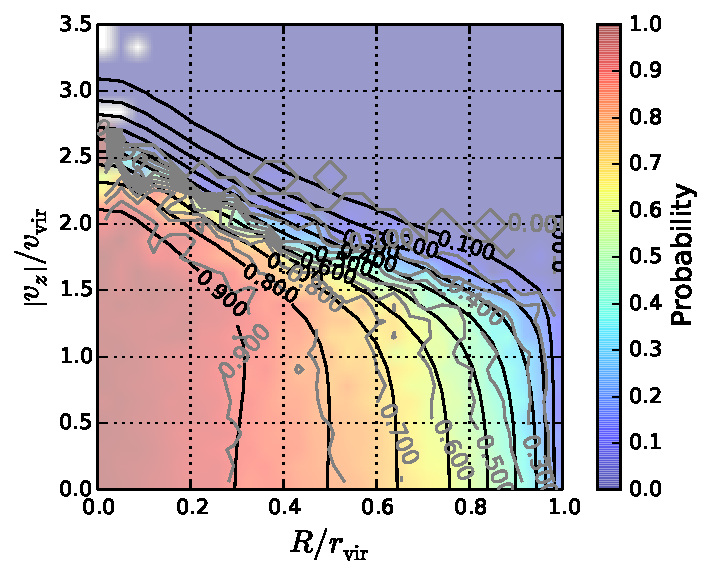
\includegraphics[width=0.6\linewidth]{figures/maggie/probabilities.pdf}
    \caption{The probability contours from the simulation of \citet{Borgani+01}
        and our model. In \emph{gray} the contours obtained with particles from
        the cosmological simulation, and in \emph{black} the theoretical
        expectation from \bartrefequation{gi_over_gh}. The color scale reflects
        the probability from the simulation. The theoretical probability agree
        with the cosmological simulation except for high velocities along the
        line-of-sight, in part explained by the lack of particles with such
        velocities, giving a bad constraint for the probability to be in the
        halo from the simulation.
\label{fig:probabilities}}
\end{figure}

\remark{%
    We can first think that the observed discrepancies in
    \bartreffigure{probabilities} are the consequence of a bad choice for the
    ratio $a/b$ (see \bartrefappendix{profiles}) or for the concentration, but
    changing this values doesn't reduce them. The contours for the simulation
    seem to show a cut-off in the line-of-sight velocity dispersion for high
    velocities, like if the distribution is truncated above a given velocity. A
    functional form with such a property is the generalization of the Gaussian
    called the $q$-Gaussian or Tsallis distribution. Assuming such a velocity
    distribution, the computation of the probability involves several
    integrals, which is CPU time consuming. Instead, we can fit a $q$-Gaussian
    on the line-of-sight velocity distribution from the simulation and
    incorporate it in the probability computation. But unfortunately, this
    doesn't solve the problem. It seems that the number of particles with high
    velocities is too low to correctly define the probability to be in the
    virial sphere of the halo, and to compare it to theoretical expectations.
    The velocity distribution isn't involved.
}

Here we assume that the density profile follow a NFW, since the dark matter
particles of the \citet{Borgani+04} simulation follow this distribution. But we
are interested in groups of galaxies and they must follow the same distribution
to apply our model. We used the galaxies from the output of the \citet{Guo+11}
semi-analytical code and checked that they follow a NFW density profile too.
But as expected, there is a bias between the galaxies and dark matter
particles. Indeed, if we fit the concentration of the NFW profile in
\citet{Guo+11} and compare it to the model of \citet{Maccio+08} obtained from
dark matter particles, we can see that the two functional are different. A
consequence is that the link between halo mass and concentration must be
adjusted for galaxies in our model. The difference between the two model of
concentration is shown in \bartreffigure{concentration_bias}.
%
\begin{figure}[ht]
    \centering
    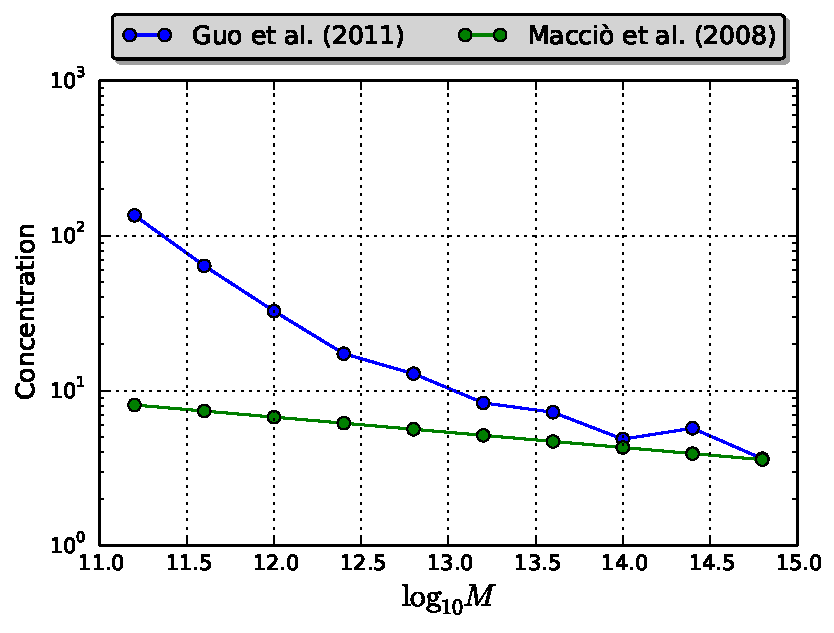
\includegraphics[width=0.8\linewidth]{figures/maggie/concentrations.pdf}
    \caption{The concentration in function of the halo mass for
        \citet{Maccio+08} in \emph{green} and fitted on the \citet{NFW+97}
        density profile of galaxies from \citet{Guo+11} with $M_r\leqslant-15$
        in \emph{blue}. The concentration of galaxies is slightly different
    from that of dark matter particles.\label{fig:concentration_bias}}
\end{figure}
%
But we note that the modulation of the concentration with the halo mass is
dependent of the cut-off in luminosity applied on the galaxy sample, making the
use of a specific density profile for galaxies inadequate. We checked the
influence of this choice on MAGGIE by comparing the performance with the
concentration from \citet{Guo+11} and from \citet{Maccio+08}. No noticeable
impact is observed in the completeness, reliability and fragmentation, except
on stellar masses and luminosities of groups but without being significant.

\section{Results on mock catalogue}
\label{sec:results_on_mock_catalogue}

\subsection{Description}
\label{sub:maggie_tests_description}

For tests we proceed as described in \citet{Yang+07, Duarte+14} and
\bartrefchapter{friends_of_friends_algorithm}. To link a selected group by the
algorithm in redshift space to the true halo in real space, we use the most
massive galaxy of the group. The true halo of a group is the true halo to which
the most massive galaxy in the selected group (referred as the central galaxy)
belongs to. With this link, we compute the completeness and reliability of
groups relatively to this halo in real space. We define statistics used to
quantify the performance of MAGGIE\@. The completeness $C$ is the fraction of
galaxies in the real space group recovered in the selected group. The
reliability $R$ is the fraction of galaxies in the selected group present in
the real space group. A primary group is defined as a selected group whose the
central galaxy match the central galaxy of the real space associated halo,
remaining groups are fragments. A complete and detailed description of the
statistics can be found in \citet{Duarte+14} and
\bartrefchapter{friends_of_friends_algorithm}.

The reliability in the case of MAGGIE is more complex since we use
probabilities for galaxies in groups. We let, with our definition, many
galaxies potentially belong to a given group. This artificially decreases
the reliability of a group because of the interlopers being systematically
considered group members with the previous definition. To take advantage of
our probabilities, let us give a new definition for the reliability. In
\citet{DM+14a}, we wrote:
%
\begin{equation}
    R=\frac{T \cap E}{E}=\frac{\sum_{i\in T\cap E}}{\sum_{i\in E}}
\end{equation}
%
But many galaxies pertains to our group with this definition and so we
weight galaxies in the previous sum by their probabilities in order to have
a coherent definition of the reliability with our probabilistic
determination of groups. Our new definition in the case of a probabilistic
galaxy group algorithm as MAGGIE is:
%
\begin{equation}
    R=\frac{T \cap E}{E}=\frac{\sum_{i\in T\cap E} p_i}{\sum_{i\in E}p_i}
\end{equation}
%
For the completeness, since the probability doesn't introduce a bias in the
selection relatively to the real group, we keep the computation as described
in \citet{DM+14a}, without weighting by probabilities.

Without probabilities, galaxies in groups form a complete partition of the
survey since groups can be seen as disjoints sets of the redshift space. But
with MAGGIE and probabilities, a galaxy can be in multiple groups so the
sets of groups are overlapping, and the \emph{dual} analysis done in
\citet{DM+14a} for the merging of real space groups can't be correctly done.
This is because the central galaxy of a real space group can be potentially
belonging to several extracted group in the redshift space.

\subsection{Optimization}

\subsection{Results}

The following tests result from the application of MAGGIE on the perfect mock
catalogue whose construction is described in \bartrefchapter{mock}. In this
case, we assume the halo mass function extracted from the Millennium-II
outputs, with a NFW density profile for galaxies identical to dark matter
particles in their halos. The influence of these assumptions will be developed
in \bartrefsection{maggie_discussions}.

We compare MAGGIE with the most popular galaxy group algorithm that is the
percolation algorithm (see \bartrefchapter{friends_of_friends_algorithm}). The
set of linking lengths used for the FoF is the one defined in~\cite{Duarte+14}
for an optimal FoF, close to the parameters used by~\cite{Robotham+11}. This
will let us see if the introduction of Bayesian model improves the galaxy
grouping compared to a simple geometrical approach as FoF.

\subsubsection{Completeness and reliability}

\begin{figure}[t]
    \centering
    \begin{minipage}{0.49\linewidth}
        \subfloat[Catalog 2]
        {%
            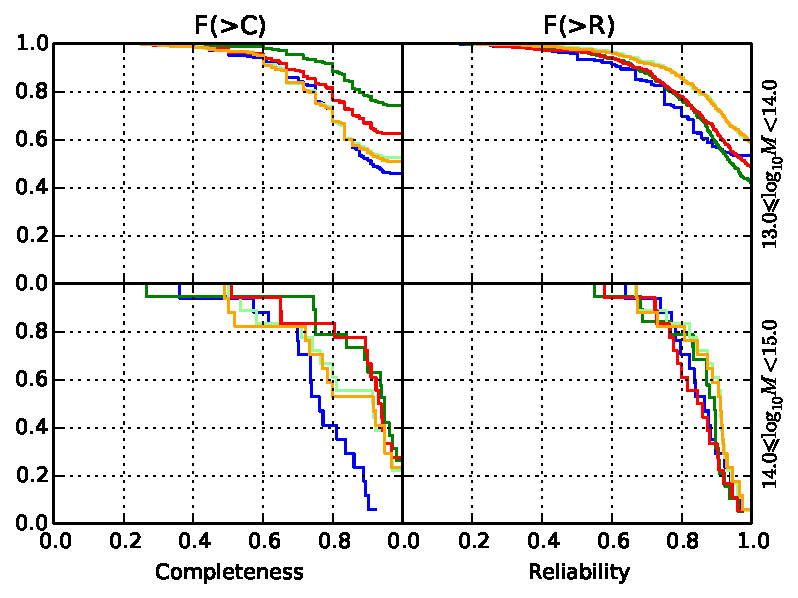
\includegraphics[width=\linewidth]{%
figures/maggie/article_fof_comparison_errors_CDF_completeness_reliability_1_article_C_R.pdf%
            }
        }
    \end{minipage}
    \begin{minipage}{0.49\linewidth}
        \subfloat[Catalog 6]
        {%
            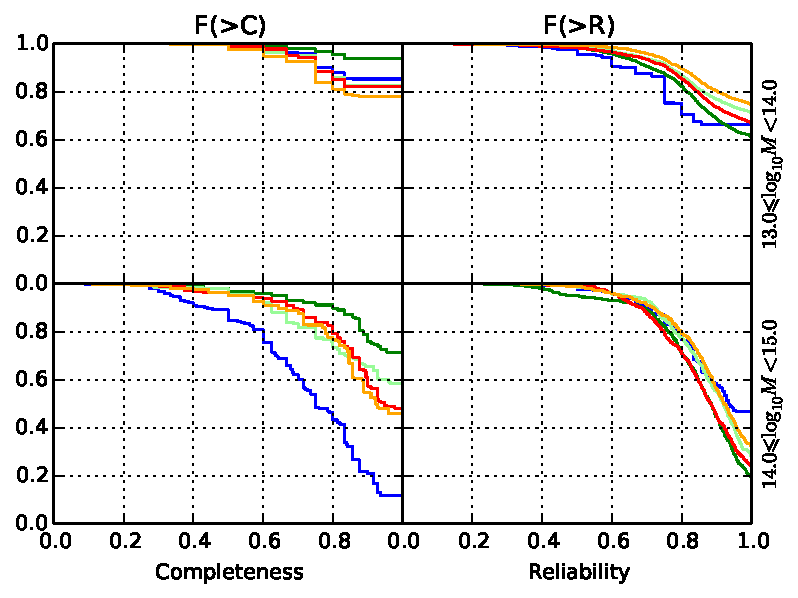
\includegraphics[width=\linewidth]{%
figures/maggie/article_fof_comparison_errors_CDF_completeness_reliability_5_article_C_R.pdf%
            }
        }
    \end{minipage}
    \caption{The cumulative distribution of the completeness $F(>C)$ and
        reliability $F(>R)$ for bins in true halo masses for two sub-samples of
        the mock catalogue. In \emph{green} MAGGIE, in \emph{red} the optimal
        FoF of \citet{Robotham+11} and in \emph{blue} the linking lengths of
    \citet{Berlind+06}. Results are shown only for primary groups (i.e.\
groups that are not fragments of real space halos).\label{fig:comp_rel}}
\end{figure}

\bartreffigure{comp_rel} shows the cumulative distribution function of the
completeness $C$ and reliability $R$ as defined in
\bartrefsubsection{maggie_tests_description} for MAGGIE and the FoF algorithm.
Results are shown only for two doubly
complete sub-samples (see \bartrefchapter{mock}), the same as in
\bartrefchapter{friends_of_friends_algorithm}. Only two bins in halo mass are
used, and we use the true halo mass, i.e.\ the virial mass of the true halo
associated to the extracted group. MAGGIE (in green) shows a better behaviour
in completeness for all masses in the two catalogue than \citet{Robotham+11}
(in blue), while the reliability is equivalent
to the optimal FoF, except for high masses for the bigger catalog.

\subsubsection{Group properties}

\begin{figure}[htb]
    \centering
    \begin{minipage}{\linewidth}
        \centering
        \begin{minipage}{\linewidth}
            \centering
            \subfloat[Differences for luminosities]
            {%
                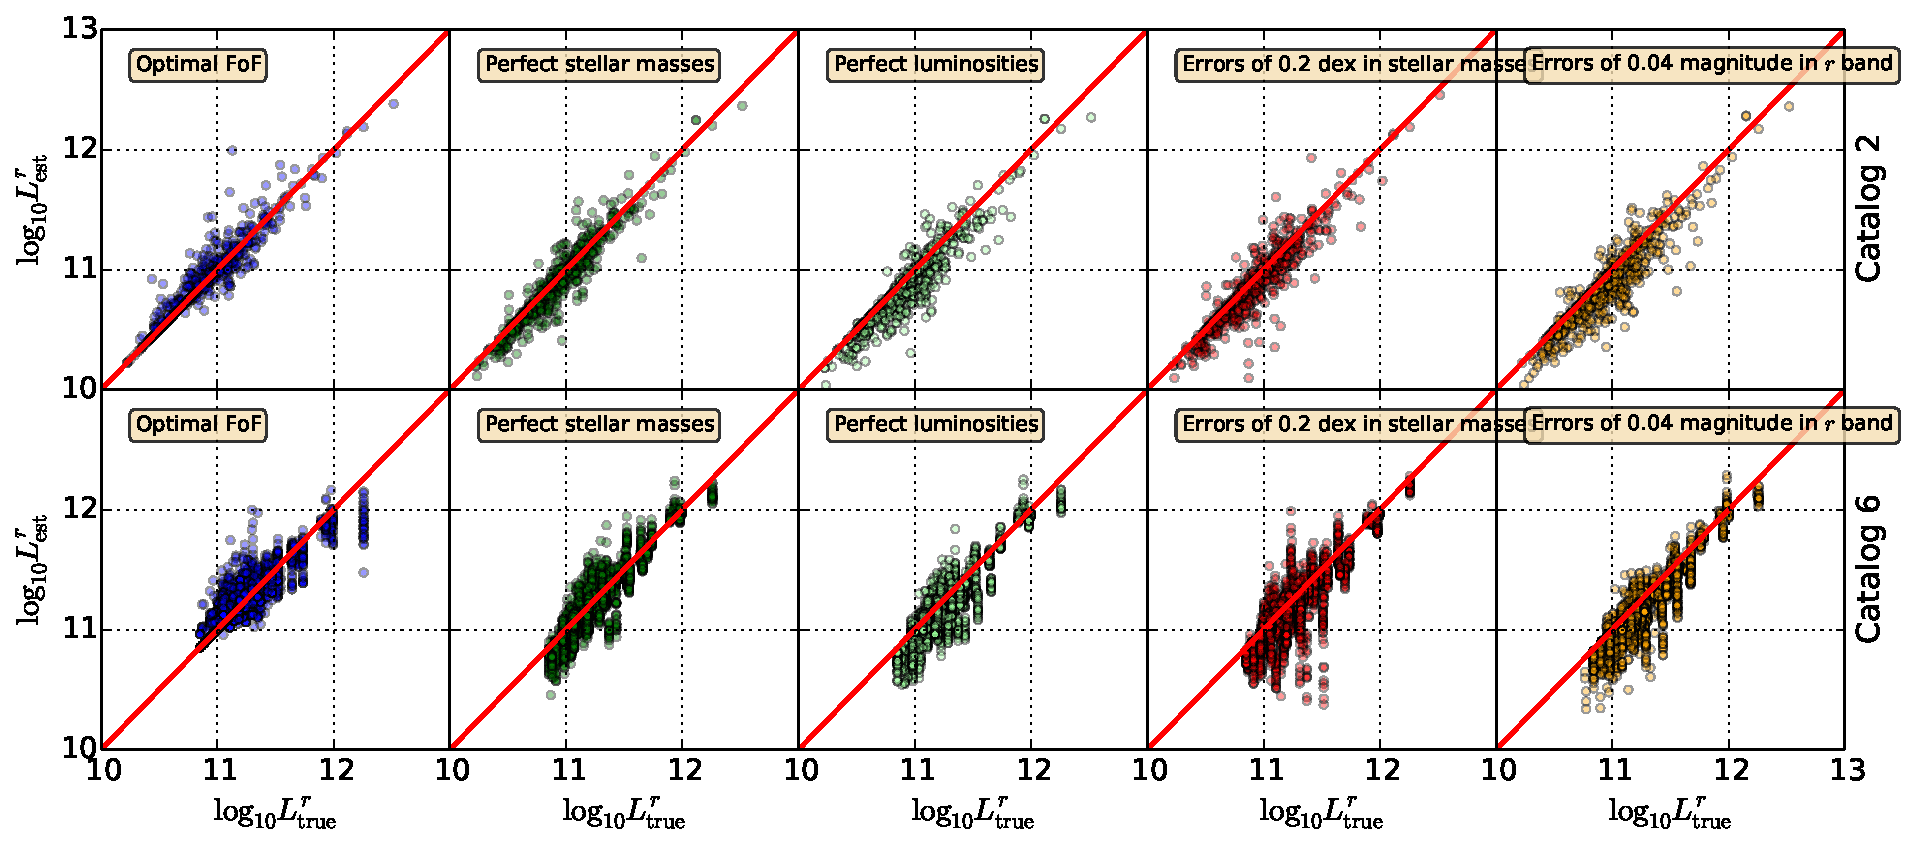
\includegraphics[width=0.8\linewidth]{%
    figures/maggie/article_fof_comparison_errors_differences_luminosity.pdf%
                }
            }
        \end{minipage}
        \begin{minipage}{\linewidth}
            \centering
            \subfloat[Differences for stellar masses]
            {%
                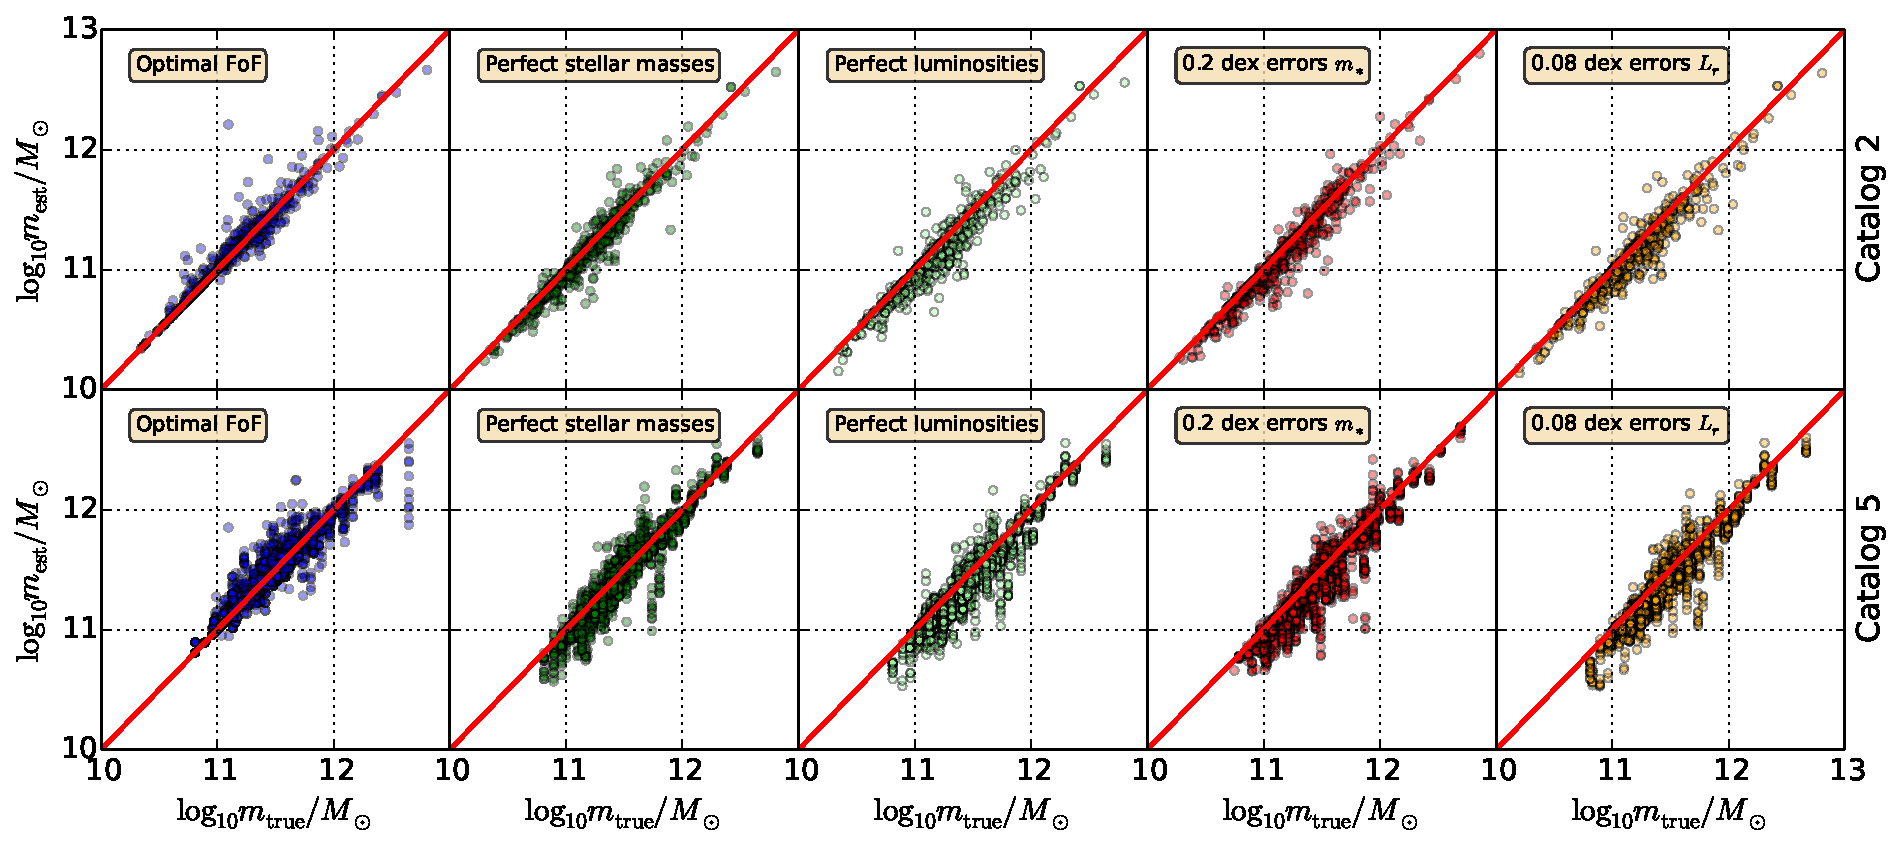
\includegraphics[width=0.8\linewidth]{%
    figures/maggie/article_fof_comparison_errors_differences_stellarmass.pdf%
                }
            }
        \end{minipage}
        \captionof{figure}{Comparison of group luminosities with the real space
        for primary groups in catalogs 2 and 6. In the top panel the difference
    on luminosities $L$ in the $r$ band. In the bottom panel, the bias and the
dispersion of the luminosity differences.\label{fig:bias_disp_lum}}
    \end{minipage}
    \begin{minipage}{\linewidth}
        \begin{minipage}{0.49\linewidth}
            \centering
            \subfloat[Bias and dispersion for luminosities]
            {%
                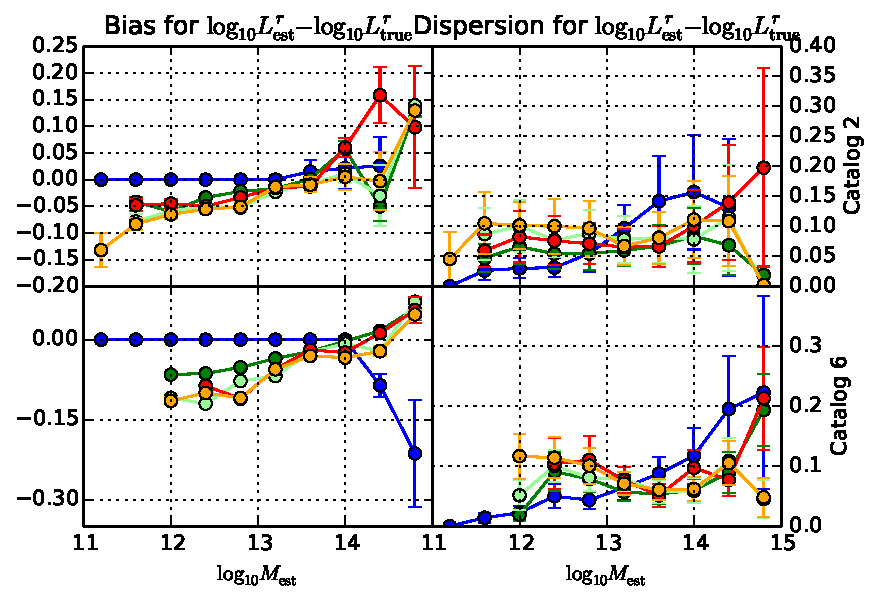
\includegraphics[width=\linewidth]{%
figures/maggie/article_fof_comparison_errors_bias_dispersion_luminosity.pdf%
                }
            }
        \end{minipage}
        \begin{minipage}{0.49\linewidth}
            \subfloat[Bias and dispersion for stellar masses]
            {%
                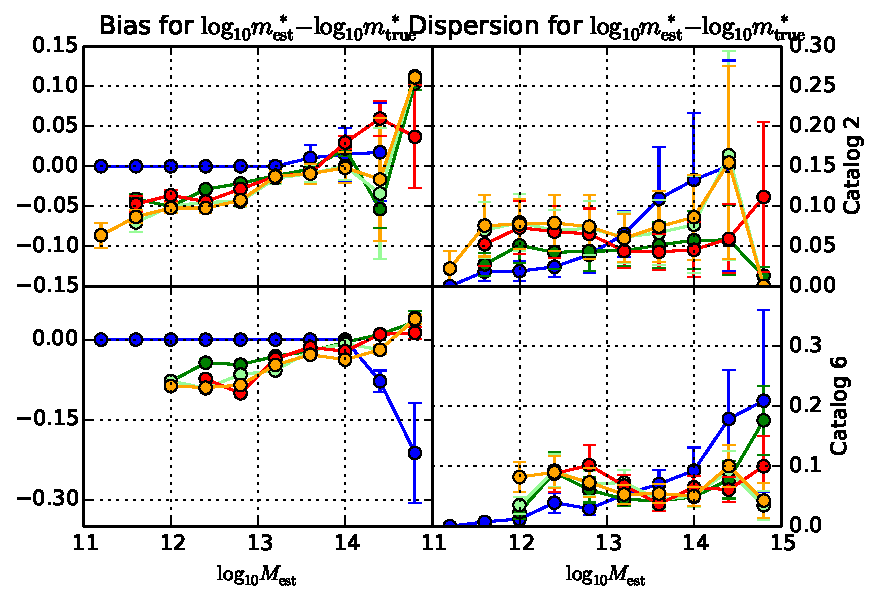
\includegraphics[width=\linewidth]{%
figures/maggie/article_fof_comparison_errors_bias_dispersion_stellarmass_bias.pdf%
                }
            }
        \end{minipage}
        \captionof{figure}{Comparison of group stellar masses with the real
        space for primary groups in catalogs 2 and 6. In the top panel the
    difference on stellar masses $m$. In the bottom panel, the bias and the
dispersion of the stellar mass differences.\label{fig:bias_disp_stellarmass}}
    \end{minipage}
\end{figure}

We test the deduced stellar mass and luminosity of selected groups for each
algorithm. For non-probabilistic FoF, they are just the sum of the galaxy
contributions. But for MAGGIE, we use the computed probabilities inside the
group to weight the stellar mass and luminosity of each galaxy. If $X$ is the
property of the group, $x_i$ the property of the galaxy $i$ in the group with
the probability $p_i$:
%
\begin{equation}
    X = \sum_i p_i x_i
\end{equation}

In \bartreffigure{bias_disp_lum}, we compare the true luminosity of groups
(computed assuming a perfect selection of groups in the sub-sample) with the
luminosity computed with the galaxy membership of each algorithm. In the bottom
panel, we show the bias and the dispersion of the difference between the true
and estimated luminosities. The \bartreffigure{bias_disp_stellarmass} is the
same for stellar masses. The optimal FoF algorithm has a lower bias than MAGGIE
since we can't observe a trend of the bias with the true halo mass, while the
dispersion is better for MAGGIE at high masses thanks to the probability
weighting that reduces the effect of interlopers.

\subsubsection{Fragmentation}

Estimating the fraction of groups in the selection that are the result of the
fragmentation of a real group is important since an observer using a group
catalog can't distinguish the primary group from the other. In
\bartreffigure{fragments}, we show the fraction of fragmented groups (defined
as in \bartrefchapter{friends_of_friends_algorithm}) in function of the
estimated halo mass. This allows to see the expected fraction of fragmented
groups by an observer using a group catalog with only information on the
estimated halo mass.

MAGGIE shows a very better behaviour in the case of the fragmentation. The
observer can be always certain that a big halo isn't the result of the
fragmentation of a true halo. This is due to the combination of the abundance
matching that gives good estimations of virial masses and the ordered search
of groups from galaxy stellar masses. But the fragmentation increases with the
decreasing estimated virial mass, since with groups of few members, it is
easier to make a mistake in the selection of the central galaxy of the group.

\subsubsection{Virial masses}
%
\begin{figure}[htb]
    \centering
    \begin{minipage}{0.49\linewidth}
        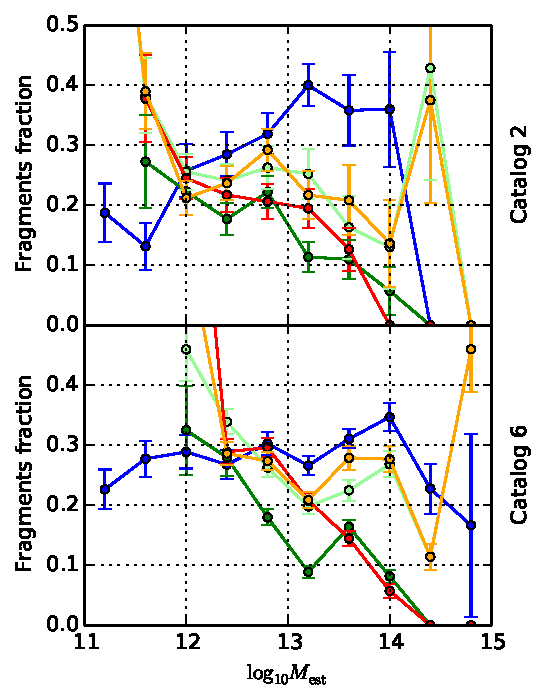
\includegraphics[width=\linewidth]{%
    figures/maggie/article_fof_comparison_errors_frag_fraction_fragments.pdf%
        }
        \captionof{figure}{The fraction of fragments according to the estimated
            halo mass of the group.\label{fig:fragments}}
    \end{minipage}
    \begin{minipage}{0.49\linewidth}
        \begin{minipage}{\linewidth}
            \subfloat[Differences for virial masses]
            {%
                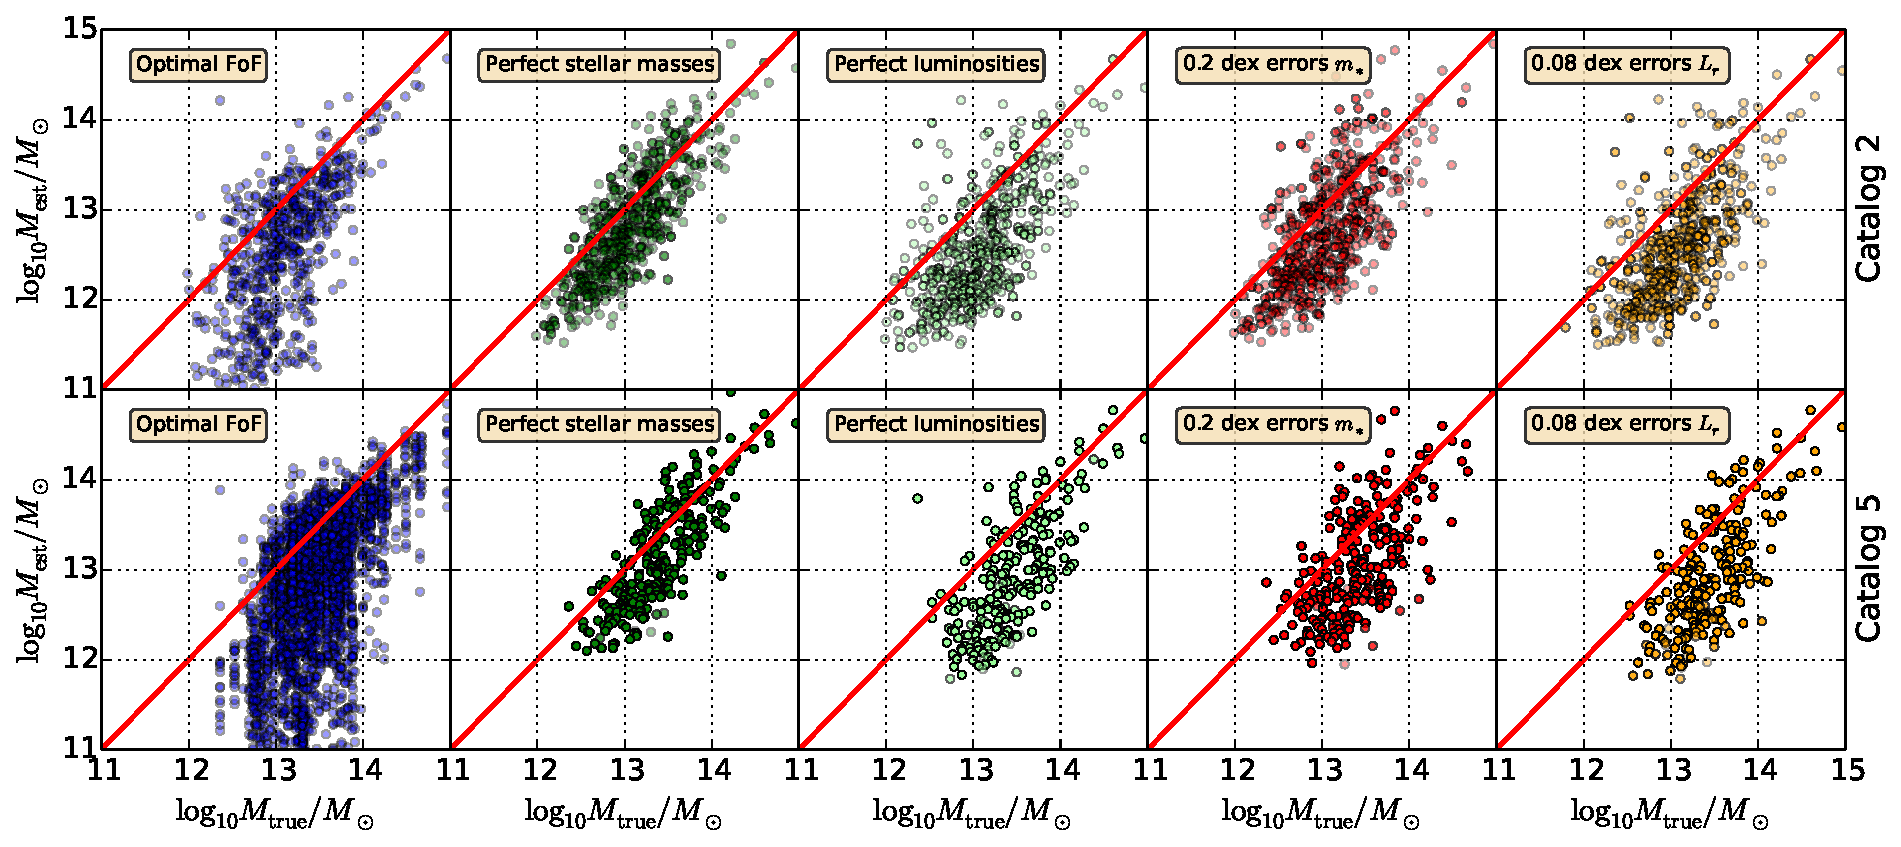
\includegraphics[width=\linewidth]{%
        figures/maggie/article_fof_comparison_errors_differences_halo_mass.pdf%
                }
            }
        \end{minipage}
        \begin{minipage}{\linewidth}
            \subfloat[Bias and dispersion for virial masses]
            {%
                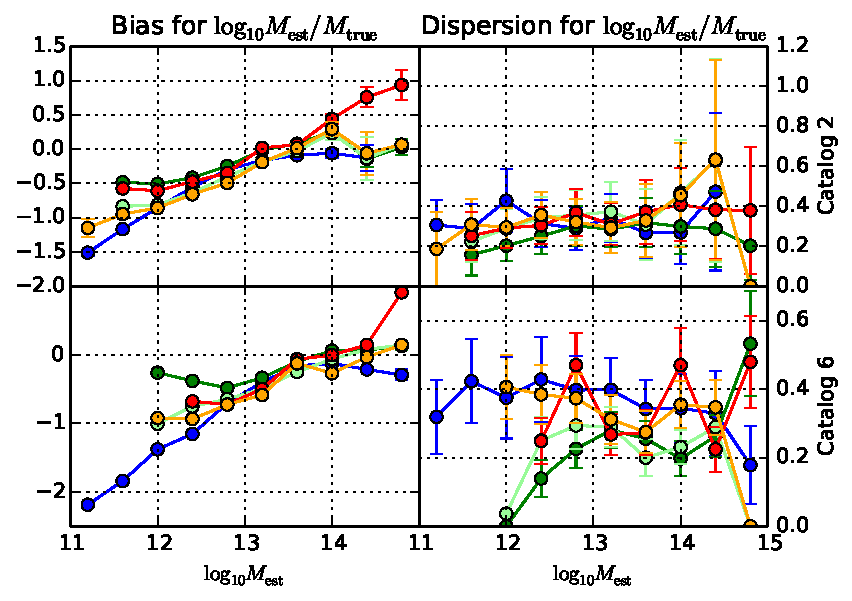
\includegraphics[width=\linewidth]{%
    figures/maggie/article_fof_comparison_errors_bias_dispersion_halo_mass.pdf%
                }
            }
        \end{minipage}
        \captionof{figure}{\label{fig:bias_disp_virial_mass}}
    \end{minipage}
\end{figure}

In \bartreffigure{bias_disp_virial_mass}, we compare the estimation of the
virial mass by application of the virial theorem for FoF algorithm and by
abundance matching for MAGGIE\@. As we already discussed, the virial theorem
isn't very suitable in recovering the virial masses of groups when they have a
small mass (between $10^{12}$ and $10^{13}M_\odot$). We can't really see it in
the bias of the estimation between the two algorithms, but the difference is
pronounced in the dispersion where MAGGIE has a very good behaviour except for
high virial masses (around $10^{15}M_\odot$) as we expected because of the
choice of the relation for the abundance matching (see
\bartrefsubsection{hmf_test}). At this mass regime, the virial theorem improves
the estimation by the presence of more numerous galaxies putting less
uncertainties in the velocity dispersion of the group. Hence, a relative good
completeness in the group leads to a more precise virial mass.

\section{Discussions}
\label{sec:maggie_discussions}

A simple comparison of MAGGIE with the most popular and geometrical grouping
algorithm shows that MAGGIE is well adapted in recovering galaxy groups from
redshift space catalogues. Extracted global properties of groups are less
biased and catastrophic cases avoided by using probabilities as weights to
smooth the estimation. The membership inside these groups is better too since
the completeness shows that MAGGIE selects a large part of galaxies from the
real group, without polluting it by interlopers (as shown by the reliability).
Moreover, the importance of interlopers is reduced still by using
probabilities. The abundance matching technique is also a very good way to
contribute to this galaxy group extraction, since the virial mass estimation
relies only on group or galaxy properties, which are observables certainly
biased and uncertain, but with less importance than biased geometrical
informations (velocity dispersion, richness\ldots). On the contrary geometrical
informations perform well when the number of galaxies is important because
interlopers act as a small noise in the group membership, even with their
relative important presence at high halo masses for the FoF algorithm. Hence,
velocity dispersion and harmonic radius are not very biased and the virial
theorem becomes good.

This comparison is done in the case where the data on galaxies is perfect, in
the sense that there are no observational errors and we perfectly know the
various scaling relations used in our models. But the behaviour of MAGGIE is
unknown in the real situation of an observer, with a limited knowledge in these
models. In the following sections, we study the robustness of the performance
of MAGGIE under pertubations, i.e.\ in cases where we make some modifications
in the halo mass function, the galaxy luminosities and stellar masses\ldots, as
in studies of equilibriums.

\subsection{Prior halo mass --- central stellar mass relation}
\label{sub:prior_relation}

We tested the choice for the initial relation between the halo mass and the
central stellar mass of groups to see its effects on MAGGIE\@. We used the
relation from \citet{BCW+10} against a simple ratio relation with different
values for the ratio. Extracted groups are insensitive to this choice, if we
keep this choice with physical values. The iterative process corrects a bad
assumption in our initial guess.

\subsection{Influence of the halo mass function model}
\label{sub:hmf_test}

The estimation of the virial mass is an important aspect. Halo masses are
linked to the global environment of galaxies and a biased estimation will
affect observed trends of galaxy properties with the environment.

Our mass computation needs to be precise in the larger mass range possible, and
independent of polluted environment of groups by some interlopers. The
abundance matching technique seems to be a good way to estimate the virial mass
of galaxy group halos. In principle, it seems more biased than using the
luminosities or stellar masses of groups, but since the central galaxy in a
selected group is well recovered, this is a quantity less affected by
interlopers and so the halo mass estimation will be good enough. But since
there is a saturation of the relation between the halo mass and the central
stellar mass at high halo mass, we expect that the estimation will be poorer
for high masses than other methods.

The majority of the halo mass function described in the literature fit the FoF
mass of the halos instead of the spherical over-density mass, which is related
to the virial mass of the halo. Since we used the galaxy catalogue from
\citet{Guo+11} whose semi-analytical code was applied onto the Millennium-II
run, we fit the virial halo mass function directly on its output.
%
\begin{figure}[t]
    \centering
    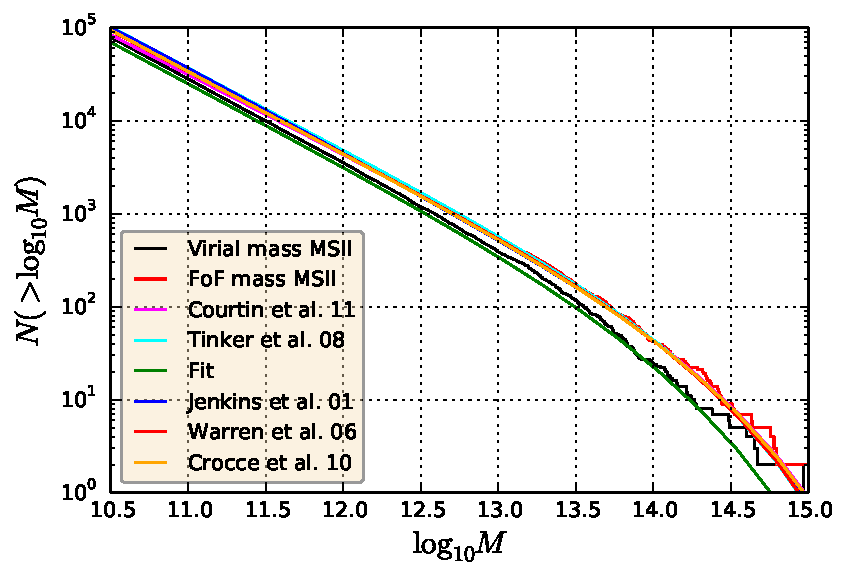
\includegraphics[width=0.6\linewidth]{figures/maggie/hmf.pdf}
    \caption{Cumulative halo mass function for the output of the Millennium-II
    run for FoF masses (red) and virial masses (black), and some models of halo
mass functions. We show the fit we have done on the virial mass function
(green).\label{fig:hmf}}
\end{figure}
%
We show it in \bartreffigure{hmf} where we plot the FoF mass function (in red)
and the virial mass function (in black) for halos in the Millennium-II
simulations at redshift zero. Virial masses are lower than FoF masses so we
don't use existing models of halo mass functions displayed too on the figure.
The way of computing such halo mass function is described in
\bartrefappendix{halo_mass_functions}.

\begin{figure}[htbp]
    \centering
    \begin{minipage}{\linewidth}
        \centering
        \begin{minipage}{0.49\linewidth}
            \subfloat[Catalogue 2]{%
                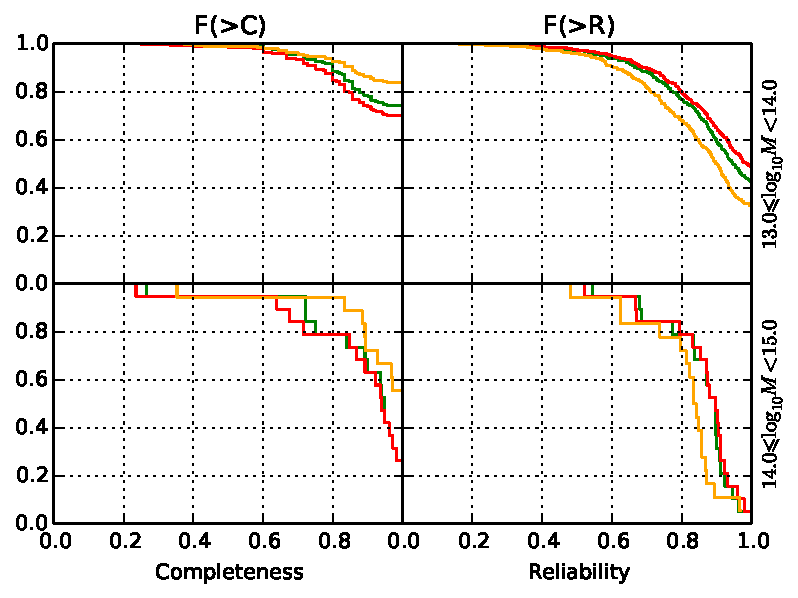
\includegraphics[width=\linewidth]{%
figures/maggie/msii_courtin_warren_CDF_completeness_reliability_1_article_C_R.pdf%
                }
            }
        \end{minipage}
        \begin{minipage}{0.49\linewidth}
            \subfloat[Catalogue 6]{%
                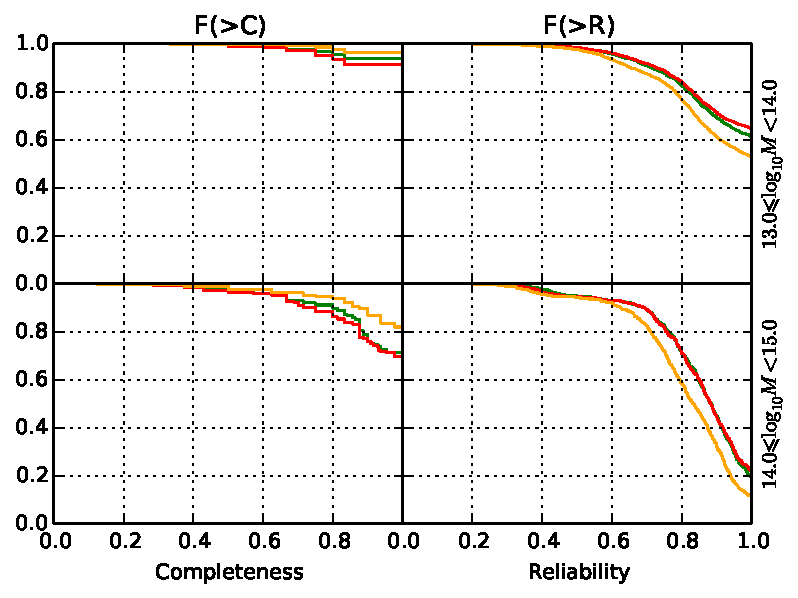
\includegraphics[width=\linewidth]{%
figures/maggie/msii_courtin_warren_CDF_completeness_reliability_5_article_C_R.pdf%
                }
            }
        \end{minipage}
        \captionof{figure}{Errors for the choice of the halo mass
        function.\label{fig:cdf_hmf}}
    \end{minipage}
    \begin{minipage}{\linewidth}
        \centering
        \begin{minipage}{0.49\linewidth}
            \subfloat[Group halo masses]{%
                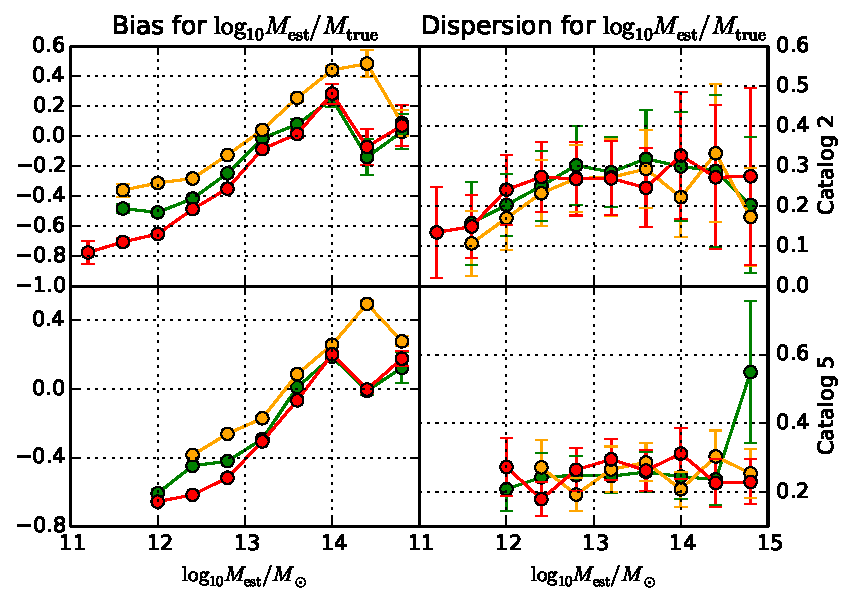
\includegraphics[width=\linewidth]{%
            figures/maggie/msii_courtin_warren_bias_dispersion_halo_mass.pdf%
                }
            }
        \end{minipage}
        \begin{minipage}{0.49\linewidth}
            \subfloat[Group stellar masses]{%
                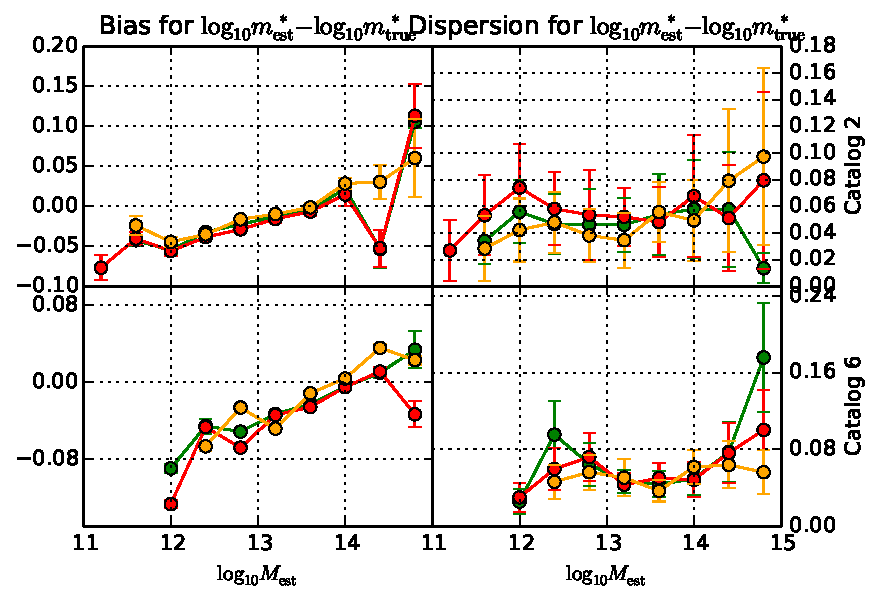
\includegraphics[width=\linewidth]{%
            figures/maggie/msii_courtin_warren_bias_dispersion_stellarmass.pdf%
                }
            }
        \end{minipage}
        \begin{minipage}{0.49\linewidth}
            \subfloat[Group luminosities]{%
                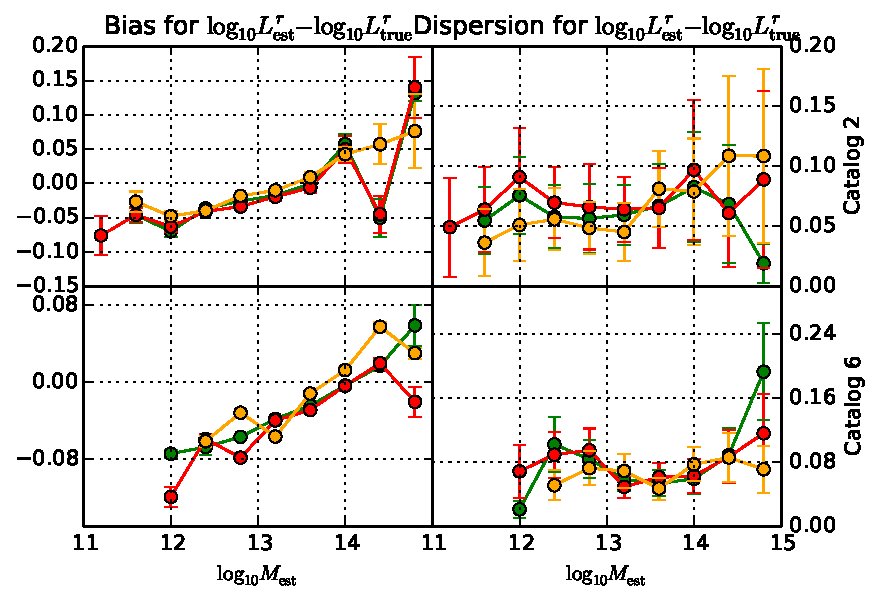
\includegraphics[width=\linewidth]{%
            figures/maggie/msii_courtin_warren_bias_dispersion_luminosity.pdf%
                }
            }
        \end{minipage}
        \captionof{figure}{Errors for the choice of the halo mass
        function.\label{fig:bias_disp_hmf}}
    \end{minipage}
\end{figure}

The robustness of MAGGIE against the choice of the halo mass function is
important because this choice will affect the completeness and reliability of
our selected groups and their properties too in a non obvious way. Indeed, the
halo mass function is a prior in MAGGIE and doesn't reflect necessary the
reality. We apply an equivalent of the perturbation method to test the
stability of MAGGIE under a bad choice of model. We used two halo mass
functions very different of the true one: \citet{Warren+06} and
\citet{Courtin+11}. Those models are fits of the FoF halo mass function from
different cosmological simulations. This is not the same as the virial mass but
ideal for perturbation test. The result of the application of MAGGIE with the
these models is shown in \bartreffigure{cdf_hmf} and
\bartreffigure{bias_disp_hmf}.

Comparisons are performed against the perfect case of MAGGIE (in green) with
the halo mass function directly fitted on the Millennium-II, perfect stellar
masses and luminosities for galaxies. In orange, halo mass function of
\citet{Warren+06} and in red, that one of \citet{Courtin+11}. The influence of
the halo mass function is very small on the completeness and reliability for
all catalogues and for group properties.
\com{What to say more?}

\subsection{Influence of the cosmology}

Our problematic is still the same: as an observer, we don't know the real space
and its properties. So, we assume a given set of cosmological parameters. When
applying group finders on our mock catalog, we use the cosmology of the
simulation from which are constructed our mock. But in reality, we know those
parameters with a given uncertainty and we want to know their effects on the
group extraction.

To answer this question, we must know where the cosmology is relevant in the
algorithm. For example, when computing the projected radius of a galaxy at the
redshift of the group, we implicitly need to compute the luminosity distance
which is cosmology dependent. We assume in our case a flat Universe and in this
case, it is computed using just elliptic integrals
\citep{Liu+11,Eisenstein+97}. So cosmological parameters have an influence on
this distance, and in consequence, on the membership of galaxy groups.
Moreover, the halo mass function is dependent of the cosmology assumed by the
observer for many models and can affect the virial mass estimations. In our
case, the halo mass function is fitted on the real space data and its influence
can't be really measured. But we expect it has the same influence as a bad
choice for the halo mass function. We ran MAGGIE with the true cosmology (from
Millennium-II simulation) and two false cosmology with respect to our mock
catalog (Planck and WMAP9) to compare results. As expected, the importance of
the cosmology is low, of the order of statistical errors, as seen in
\bartreffigure{cdf_cosmology} and \bartreffigure{bias_disp_cosmology}.
%
\begin{figure}[htbp]
    \centering
    \begin{minipage}{\linewidth}
        \centering
        \begin{minipage}{0.49\linewidth}
            \subfloat[Catalogue 2]{%
                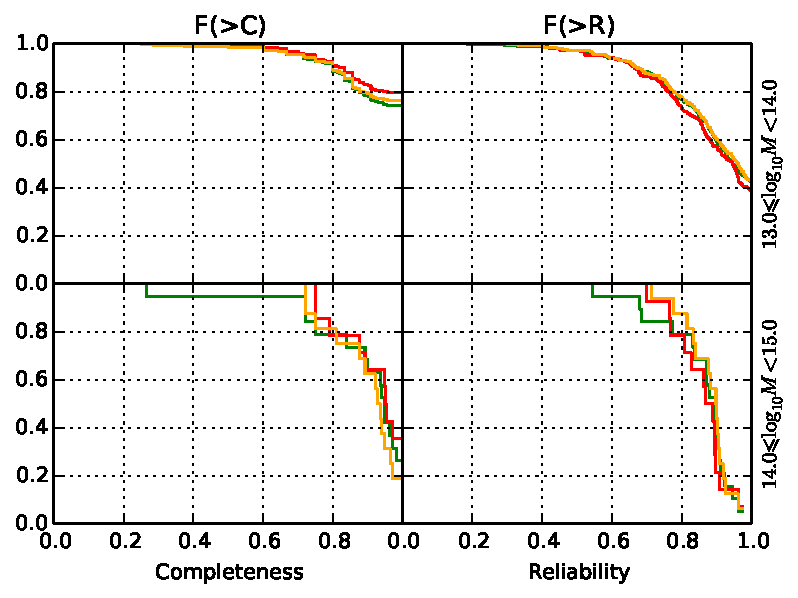
\includegraphics[width=\linewidth]{%
figures/maggie/planck_wmap9_CDF_completeness_reliability_1_article_C_R.pdf%
                }
            }
        \end{minipage}
        \begin{minipage}{0.49\linewidth}
            \subfloat[Catalogue 6]{%
                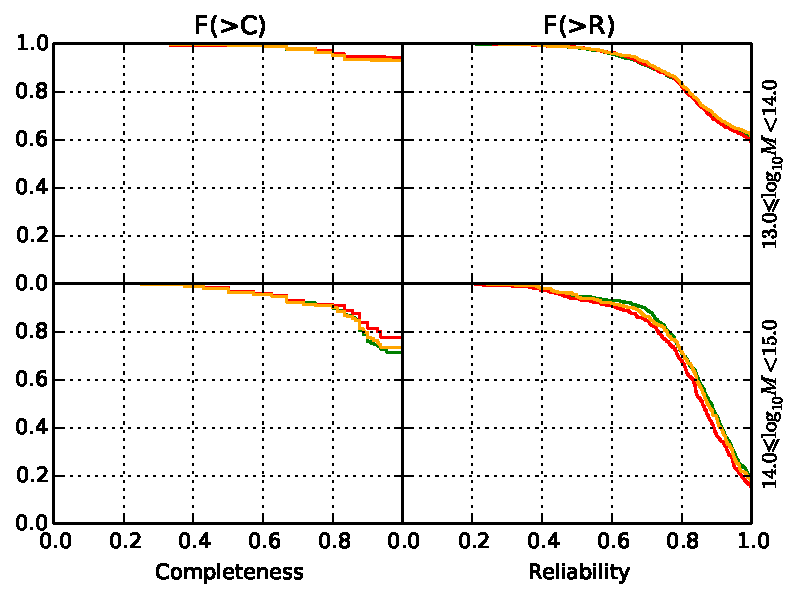
\includegraphics[width=\linewidth]{%
figures/maggie/planck_wmap9_CDF_completeness_reliability_5_article_C_R.pdf%
                }
            }
        \end{minipage}
        \captionof{figure}{Errors for the choice of the
        cosmology.\label{fig:cdf_cosmology}}
    \end{minipage}
    \begin{minipage}{\linewidth}
        \centering
        \begin{minipage}{0.49\linewidth}
            \subfloat[Group halo masses]{%
                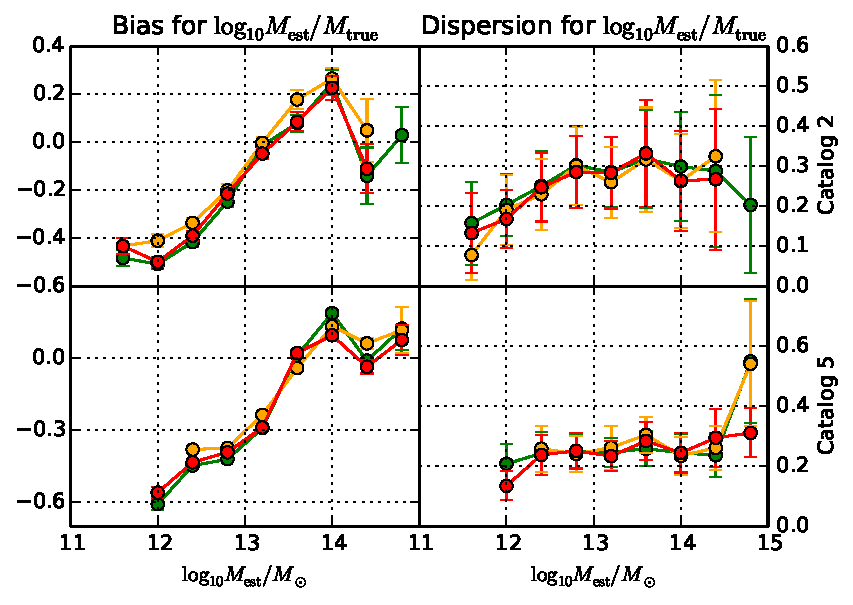
\includegraphics[width=\linewidth]{%
                figures/maggie/planck_wmap9_bias_dispersion_halo_mass.pdf%
                }
            }
        \end{minipage}
        \begin{minipage}{0.49\linewidth}
            \subfloat[Group stellar masses]{%
                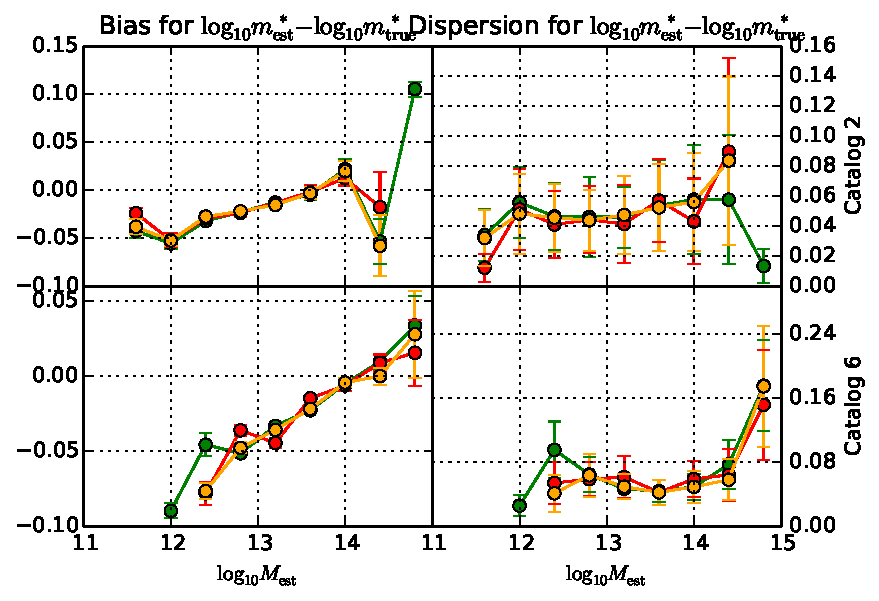
\includegraphics[width=\linewidth]{%
                figures/maggie/planck_wmap9_bias_dispersion_stellarmass.pdf%
                }
            }
        \end{minipage}
        \begin{minipage}{0.49\linewidth}
            \subfloat[Group luminosities]{%
                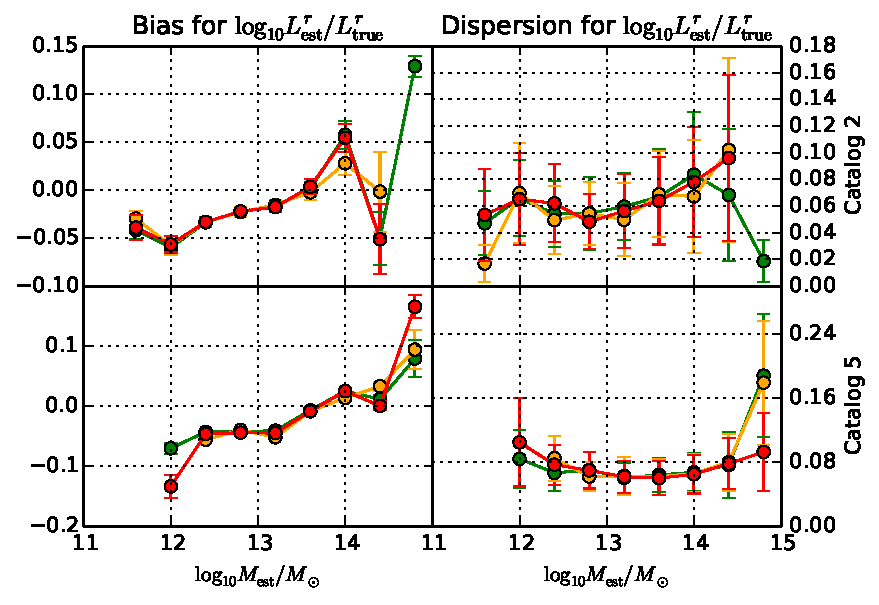
\includegraphics[width=\linewidth]{%
                figures/maggie/planck_wmap9_bias_dispersion_luminosity.pdf%
                }
            }
        \end{minipage}
        \caption{Errors for the choice of the
        cosmology.\label{fig:bias_disp_cosmology}}
    \end{minipage}
\end{figure}

\subsection{Influence of observational errors}
\label{sub:observational_errors}

Our way of sorting galaxies by mass uses our prior on the galaxy formation
scenario. Indeed, the stellar mass of the central galaxy of a dark matter halo
is correlated to its virial mass. But the relation is saturated at high halo
masses. So the intrinsic precision is affected by this choice.

Moreover, the estimation of stellar masses from the observations and spectrum
is not very precise and can significantly differ according to the way of
computing it. We show the differences between some models present in the SDSS
data base, with the bias and dispersion for each distribution, in
\bartrefchapter{sdss}. Typically, the errors in the estimation is roughly 0.3
dex. We introduce such errors in the stellar masses of the mock catalogue to
estimate the effect of the bad estimation. We generated Gaussian errors without
bias and dispersion of 0.3, 0.5, 0.9 dex. The effect of an error on stellar
masses is quite catastrophic in the completeness and the dispersion of group
properties, while bias is unaffected since we didn't introduced one.

We should use an other tracer for the halo mass as the central luminosity,
which is less affected by observational errors. Indeed, the principal
sources of errors in the computation of the absolute magnitude of a galaxy
are the photometry, the extinction and K-correction, and the redshift
through the distance modulus:
%
\begin{equation}
    \Delta M=\Delta m + \frac{5}{\ln{10}}
    \frac{\Delta d_\mathrm{lum} \left(z\right)}{\Delta z}
    \frac{1}{d_\mathrm{lum} \left(z\right)} + \Delta E + \Delta K\left(z\right)
\end{equation}
%
$\Delta m$ is of the order of $10^{-2}$ in the SDSS, the second term is
between $10^{-4}$ and $10^{-2}$ in the range of redshift used for the
catalogues. The K-correction, if we follow the method of
\citet{Chilingarian+10}, is of the order of $10^{-2}$. There is the problem
of the extinction for which the precision can't be really estimated.
Moreover, peculiar velocities worst the situation since they contribute to
the computation of the distance modulus. But for non-nearby galaxies and
globally, the errors should be small.

Intrinsically, using luminosities instead of stellar masses in the inference
of group virial masses is expected to be less precise because the relation
between the luminosity of the central galaxy and the halo mass is more
saturated for high mass groups. But the gain is in the precision and the
robustness relatively to the precision.

\section{Application to SDSS}
\label{sec:application_to_sdss}

% vim: set tw=79 ft=tex:
